\tikzset{every picture/.style={line width=0.75pt}}  

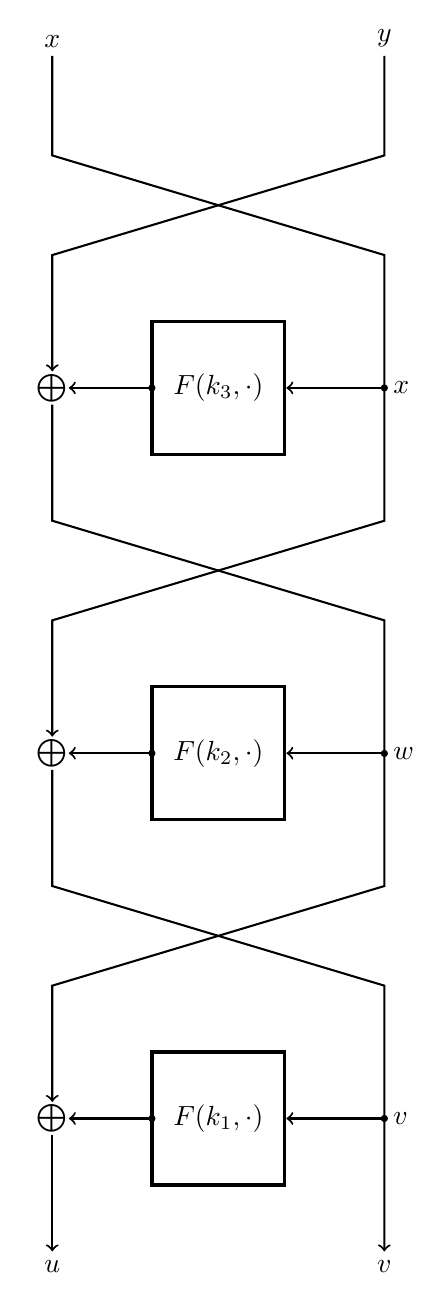
\begin{tikzpicture}[x=0.75pt,y=0.75pt,yscale=-0.8,xscale=0.8]


\draw  [line width=1.2]  (80,200) -- (160,200) -- (160,280) -- (80,280) -- cycle ;
\draw  [line width=1.2]  (80,420) -- (160,420) -- (160,500) -- (80,500) -- cycle ;
\draw  [line width=1.2]  (80,640) -- (160,640) -- (160,720) -- (80,720) -- cycle ;

\draw  [->]  (20,40) -- (20,100) -- (220,160) -- (220,320) -- (20,380) -- (20,450) ;
\draw  [->]  (20,470) -- (20,540) -- (220,600) -- (220,760) ;
\draw  [->]  (220,40) -- (220,100) -- (20,160) -- (20,230) ;
\draw  [->]  (20,250) -- (20,320) -- (220,380) -- (220,540) -- (20,600) -- (20,670) ;
\draw  [->]  (20,690) -- (20,760) ;

\draw  [->]  (80,240) -- (30,240) ;
\draw  [->]  (220,240) -- (161,240) ;
\draw  [->]  (80,460) -- (30,460) ;
\draw  [->]  (220,460) -- (161,460) ;
\draw  [->]  (80,680) -- (30,680) ;
\draw  [->]  (220,680) -- (161,680) ;

\draw  [fill={rgb, 255:red, 0; green, 0; blue, 0 }  ,fill opacity=1 ] (218.5,240) .. controls (218.5,239.17) and (219.17,238.5) .. (220,238.5) .. controls (220.83,238.5) and (221.5,239.17) .. (221.5,240) .. controls (221.5,240.83) and (220.83,241.5) .. (220,241.5) .. controls (219.17,241.5) and (218.5,240.83) .. (218.5,240) -- cycle ;
\draw  [fill={rgb, 255:red, 0; green, 0; blue, 0 }  ,fill opacity=1 ] (78.5,240) .. controls (78.5,239.17) and (79.17,238.5) .. (80,238.5) .. controls (80.83,238.5) and (81.5,239.17) .. (81.5,240) .. controls (81.5,240.83) and (80.83,241.5) .. (80,241.5) .. controls (79.17,241.5) and (78.5,240.83) .. (78.5,240) -- cycle ;
\draw  [fill={rgb, 255:red, 0; green, 0; blue, 0 }  ,fill opacity=1 ] (78.5,460) .. controls (78.5,459.17) and (79.17,458.5) .. (80,458.5) .. controls (80.83,458.5) and (81.5,459.17) .. (81.5,460) .. controls (81.5,460.83) and (80.83,461.5) .. (80,461.5) .. controls (79.17,461.5) and (78.5,460.83) .. (78.5,460) -- cycle ;
\draw  [fill={rgb, 255:red, 0; green, 0; blue, 0 }  ,fill opacity=1 ] (218.5,460.15) .. controls (218.5,459.33) and (219.17,458.65) .. (220,458.65) .. controls (220.83,458.65) and (221.5,459.33) .. (221.5,460.15) .. controls (221.5,460.98) and (220.83,461.65) .. (220,461.65) .. controls (219.17,461.65) and (218.5,460.98) .. (218.5,460.15) -- cycle ;
\draw  [fill={rgb, 255:red, 0; green, 0; blue, 0 }  ,fill opacity=1 ] (218.5,680) .. controls (218.5,679.17) and (219.17,678.5) .. (220,678.5) .. controls (220.83,678.5) and (221.5,679.17) .. (221.5,680) .. controls (221.5,680.83) and (220.83,681.5) .. (220,681.5) .. controls (219.17,681.5) and (218.5,680.83) .. (218.5,680) -- cycle ;
\draw  [fill={rgb, 255:red, 0; green, 0; blue, 0 }  ,fill opacity=1 ] (78.5,680) .. controls (78.5,679.17) and (79.17,678.5) .. (80,678.5) .. controls (80.83,678.5) and (81.5,679.17) .. (81.5,680) .. controls (81.5,680.83) and (80.83,681.5) .. (80,681.5) .. controls (79.17,681.5) and (78.5,680.83) .. (78.5,680) -- cycle ;

\draw (20,240) node  [font=\large]  {$\bigoplus $};
\draw (20,460) node  [font=\large]  {$\bigoplus $};
\draw (20,680) node  [font=\large]  {$\bigoplus $};
\draw (120,240) node    {$F( k_{3} ,\cdot )$};
\draw (120,460) node    {$F( k_{2} ,\cdot )$};
\draw (120,680) node    {$F( k_{1} ,\cdot )$};
\draw (20,36.6) node [anchor=south] [inner sep=0.75pt]    {$x$};
\draw (220,36.6) node [anchor=south] [inner sep=0.75pt]    {$y$};
\draw (223.5,240) node [anchor=west] [inner sep=0.75pt]    {$x$};
\draw (223.5,460.15) node [anchor=west] [inner sep=0.75pt]    {$w$};
\draw (223.5,680) node [anchor=west] [inner sep=0.75pt]    {$v$};
\draw (220,763.4) node [anchor=north] [inner sep=0.75pt]    {$v$};
\draw (20,763.4) node [anchor=north] [inner sep=0.75pt]    {$u$};


\end{tikzpicture}